\documentclass{article}
\usepackage[T1]{fontenc}    % Obsługa czcionek europejskich
\usepackage[utf8]{inputenc} % Obsługa nowoczesnego kodowania znaków
\usepackage[polish]{babel}  % Ustawienia dla języka polskiego (np. dzielenie wyrazów)
\usepackage{amsmath}        % Nadal zalecane do zaawansowanej matematyki
\usepackage{graphicx} % Konieczne do grafiki

\title{Raport z Analizy Danych Iris}
\author{Data Scientist}

\begin{document} % <<-- POCZĄTEK

\maketitle

W sekcji 1 przedstawiamy analizę eksploracyjną zbioru danych Iris. Stworzyliśmy Wykres Par, aby wizualnie ocenić separowalność klas.

% --- TUTAJ ZAŁĄCZASZ OBRAZEK ---
\begin{figure}[h]
    \centering
    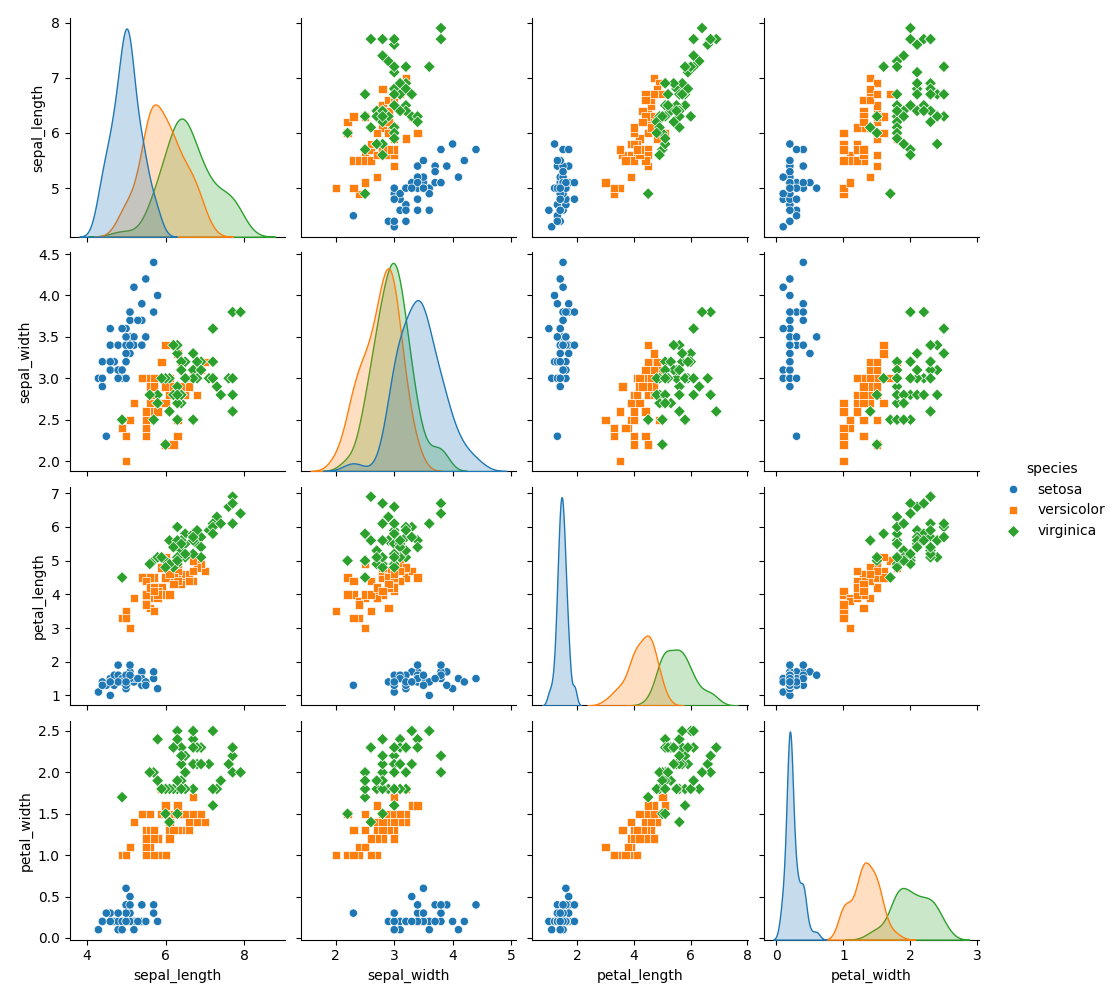
\includegraphics[width=0.9\textwidth]{pairplot_iris.png}
    \caption{Wykres Par dla zbioru danych Iris.}
    \label{fig:pairplot}
\end{figure}
% ---------------------------------

Zgodnie z Równaniem 1 (poniżej), funkcja kosztu uwzględnia regularyzację L2:

$$
J(\mathbf{w}) = \frac{1}{2m} \sum_{i=1}^{m} \left( h(\mathbf{x}^{(i)}) - y^{(i)} \right)^2 + \frac{\lambda}{2m} \sum_{j=1}^{n} w_j^2
$$

\end{document} % <<-- KONIEC

